In this part we suggest an idea to partition massive real world graphs, by first efficiently detecting communities as a way of graph coarsening and next using the clusters as the inputs of actual partitioning algorithms such as KL or FM. \\
The figure below is shown to illustrate our full pipelined approach. Label Propagation is run in the very first step on the input graph. This community detection method is utilized for clustering the nodes. The output of label propagation is then preprocessed to be used as input for the initial partitioning. After KL partitioning algorithm is run on the preprocessed data, uncoarsening is ran on the partitioned graph to recover the original nodes before community detection.
\begin{figure}[htb!]
    \centering
    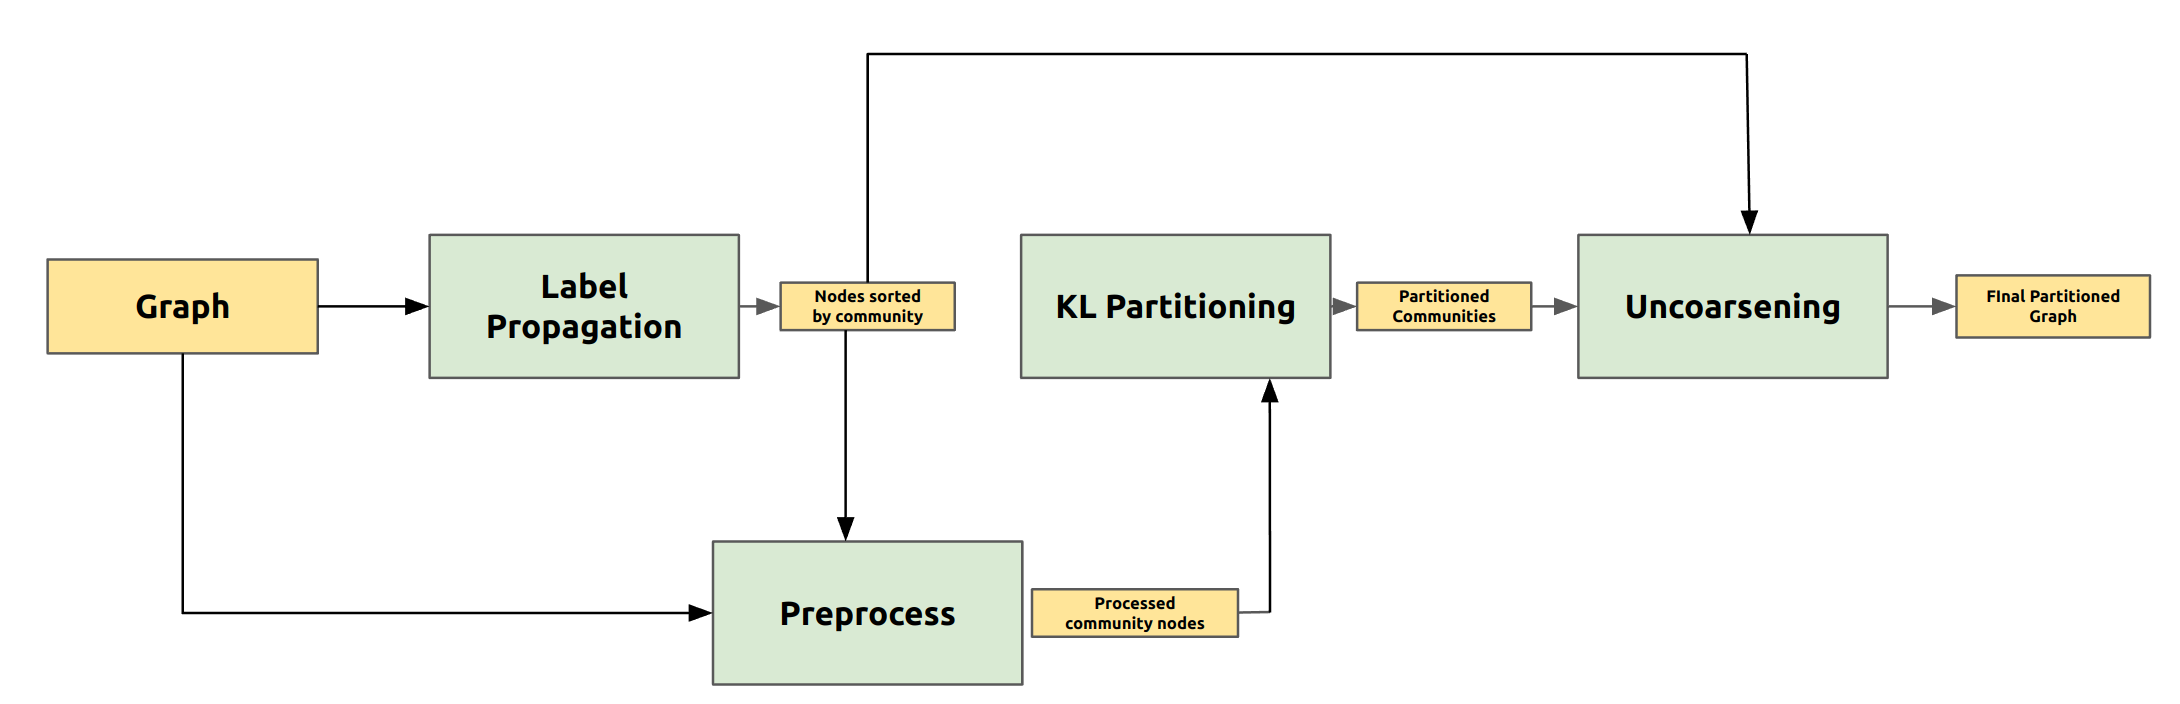
\includegraphics[width=0.9\linewidth]{FIG/full_pipeline.png}
    \caption{Full Pipeline of Our Approach}
    \label{fig:full_pipeline}
\end{figure}

Before we move on to explaining the baselines for coarsening phase, that is, detecting communities, we first show our evaluation metrics. Next, we elaborate on our proposed method in detail.
\subsection{Evaluation Metrics}
\textbf{1. Modularity} \\ \\
Graph modularity is a quality function to evaluate the compactness of communities.\\
The modularity Q is defined as:
\[ Q = \frac{1}{2m}\sum_{ij}^{}\left(A_i_j-\frac{k_ik_j}{2m}\right)\delta\left(s_i,s_j\right)\]
where $2m$ is the volume of edges, $A$ is the graph adjacency matrix, $k_i$ and $k_j$ are the edges of node $i$ and node $j$, $s_i$ and $s_j$ are the community indicator.
Modularity illustrates the difference between the actual number of edges and the expected number of edges for every pair of nodes in one community.\\
A graph is said to be modular if there exists a highest density of edges inside a community and a low density of edges between different communities. 
And as modularity can range from 0 to 1, we can interpret that higher value of Q (closer to 1) means stronger community structures. \\

\subsection{Baseline for Community Detection}
We set our baseline as the three existing community detection algorithms below. For these algorithms we used the implementation of Python library \texttt{communities} in our experiments. \\ \\
\textbf{1. Louvain Algorithm}\\ \\
Louvain algorithm gathers similar nodes or communities together into bigger clusters in the way that greedily maximizes the modularity. One pass is consisted of two phases. In phase 1, for each randomly ordered node, it is removed and inserted in a different community until no significant increase in modularity is verified. In phase 2, all nodes belonging to the same community are merged into a single giant node. \\
This method is widely used for large real world graphs. Although Louvain algorithm simplifies the process of obtaining modularity and runs in $O(nlogn)$ time, $n$ meaning the number of nodes, the calcuation of the modularity occurs every time each node is moved to a different community which leads to long computation time.\\ \\
\textbf{2. Girvan-Newman Algorithm}\\ \\
As a top-down approach, Girvan-Newman algorithm repeatedly removes 'bridge' edges with high betweenness centralities to produce more connected components, or communities. The iteration of the removal of edges terminates when the modularity value no longer increases.Edge betweenness centrality is the number of the shortest paths that go through a certain edge in the given graph. This centrality $c_{B}(e)$  is defined as \[ c_{B}(e) =  \sum_{i,j}^{}  \frac{ \sigma (i,j | e)}{\sigma(i,j)} \] where $\sigma (i,j)$ is the number of shortest paths from node \textit{i} to \textit{j} and $\sigma (i,j | e)$ is the number of shortest paths that pass through edge e.\\
The method runs in $O(m^{2}n)$ time, where \textit{m} is the number of edges and \textit{n} is the number of nodes.\\ \\
\textbf{3. Spectral Clustering}\\ \\
This method makes use of eigenvectors and eigenvalues of the adjacency matrix of the input graph to figure out the community structure. Skipping the first eigenvector, a matrix V is created which contains eigenvectors $v_{1}$, $v_{2}$, ... ,$v_{n}$ as columns. Next, the rows in matrix V are clustered using k-means into k-communities. \\
This is a NP-hard algorithm, which implies that it is unlikely to be applied on large graphs.\\

\subsection{Community detection for reducing the size of RWG} \\
Since real world graph data is huge, reducing the number of vertices of the original graph is needed. We thought that reducing the time complexity of baseline methods into nearly linear time will improve the efficiency of the overall multilevel graph partitioning. The main idea of this approach is iteratively change the label of a node based on the labels of the surrounding nodes. In this way, we can reduce the running time of the algorithm in contrast to the baseline methods, which have to compute the modularity value every iterations. \\


% Label Propagation 알고리즘
\begin{algorithm}
\caption{Label Propagation}
\label{label propagation}
\begin{algorithmic}[1]
\Procedure{Label Propagation}{$G$}
    \State Initialize the labels uniquely at all nodes in the Graph.  
    \State $t = 1$
    \State Make a list X of nodes in random order and set it to X.
    \For {each node $x$ in $X$}
        \State $C_x(t) = f(C_{x1}(t),...,C_{xim}(t),C_{xi(m+1)}(t-1),...,C_{xik}(t-1))$ 
        \State where $f$ returns the highest frequency label of neighbor nodes.
	\EndFor
	\If{Every node has their neighbors' maximum frequency label,} stop
	\ElsIf {Set $t = ${t+1} and go back to line 4} end if
\end{algorithmic}
\end{algorithm} \\

Shown in Algorithm 1, the runtime of the algorithm takes nearly linear time. Initializing all the nodes into unique labels takes $O(n)$ time, where n is the number of nodes. For each node x, deciding the label of that node depends on the label of it's neighbors, which is takes $O(d_x)$ since number of neighbors equals degree of that node x. Since this process is repeated iteratively for each node, it takes worst-case time of $O(m)$ for each node, where m is the number of total edges. \\


\subsection{Grouped clusters as the inputs for KL Algorithm} \\ 
KL is a greedy partition algorithm which takes in a graph containing nodes as input and outputs separate subsets that are connected together. The algorithm optimizes the partition by calculating the gain value in an iterative manner.\\
We expect that putting the result of label propagation into the input of Kernighan-Lin (KL) will elaborate the partitioned result and improve the accuracy of our overall pipelined algorithm.


% KL알고리즘
\begin{algorithm}
\caption{Kernighan-Lin}
\label{kernighan-lin}
\begin{algorithmic}

\Procedure{Kernighan-Lin}{$G$($V$,$E$)}
    \State This algorithms returns $G$($V$,$E$)
    \While{$g_{max} \leq 0$}
        \State $A1 :=A, B1 :=B$
        \State Compute $D$ values for all in $a$ in $A1$ and $b$ in $B1$
        %\State Let $gv, av, bv$ be empty lists
        \For {$i :=1$ to $|V|/2$}
            \State find $a[i]$ from $A1$ and $b[i]$ from $B1$, such that
                \State $g[i] = D[a[i]] + D[b[i]] -2c[a[i]][b[i]]$ is maximal
            \State remove $a[i]$ and $b[i]$ from further consideration in this pass
            \State update $D$ values for the elements of $A1 = A1 / a[i]$ and $B1 = B1 / b[i]$
        \EndFor
        \State Find $k$ which maximizes $g_{max}$, the sum of $g[1],...,g[k]$
        \If{$g_{max} > 0$} {Exchange $a[1],a[2],...,a[k]$ with $b[1],b[2],...,b[k]$}\EndWhile
\end{algorithmic}
\end{algorithm}
